
%\addcontentsline{toc}{chapter}{Anhang}
\cftaddtitleline{toc}{chapter}{Anhang}{}
\pagenumbering{Roman}
\appendix


%\chapter{Ausschreibung Bachelorarbeit}\label{anhang_ausschreibung}
% 
%\includepdf{../ressources/Projektorganisation/Ausschreibung.pdf}
%
%
%\chapter{Projektplanung}  \label{anhang_projektplan} 
%%\includepdf [landscape = true, pages=-] {../ressources/Projektorganisation/PlannungV0.pdf}
%
%\vspace*{\fill}\par
%\pagebreak

%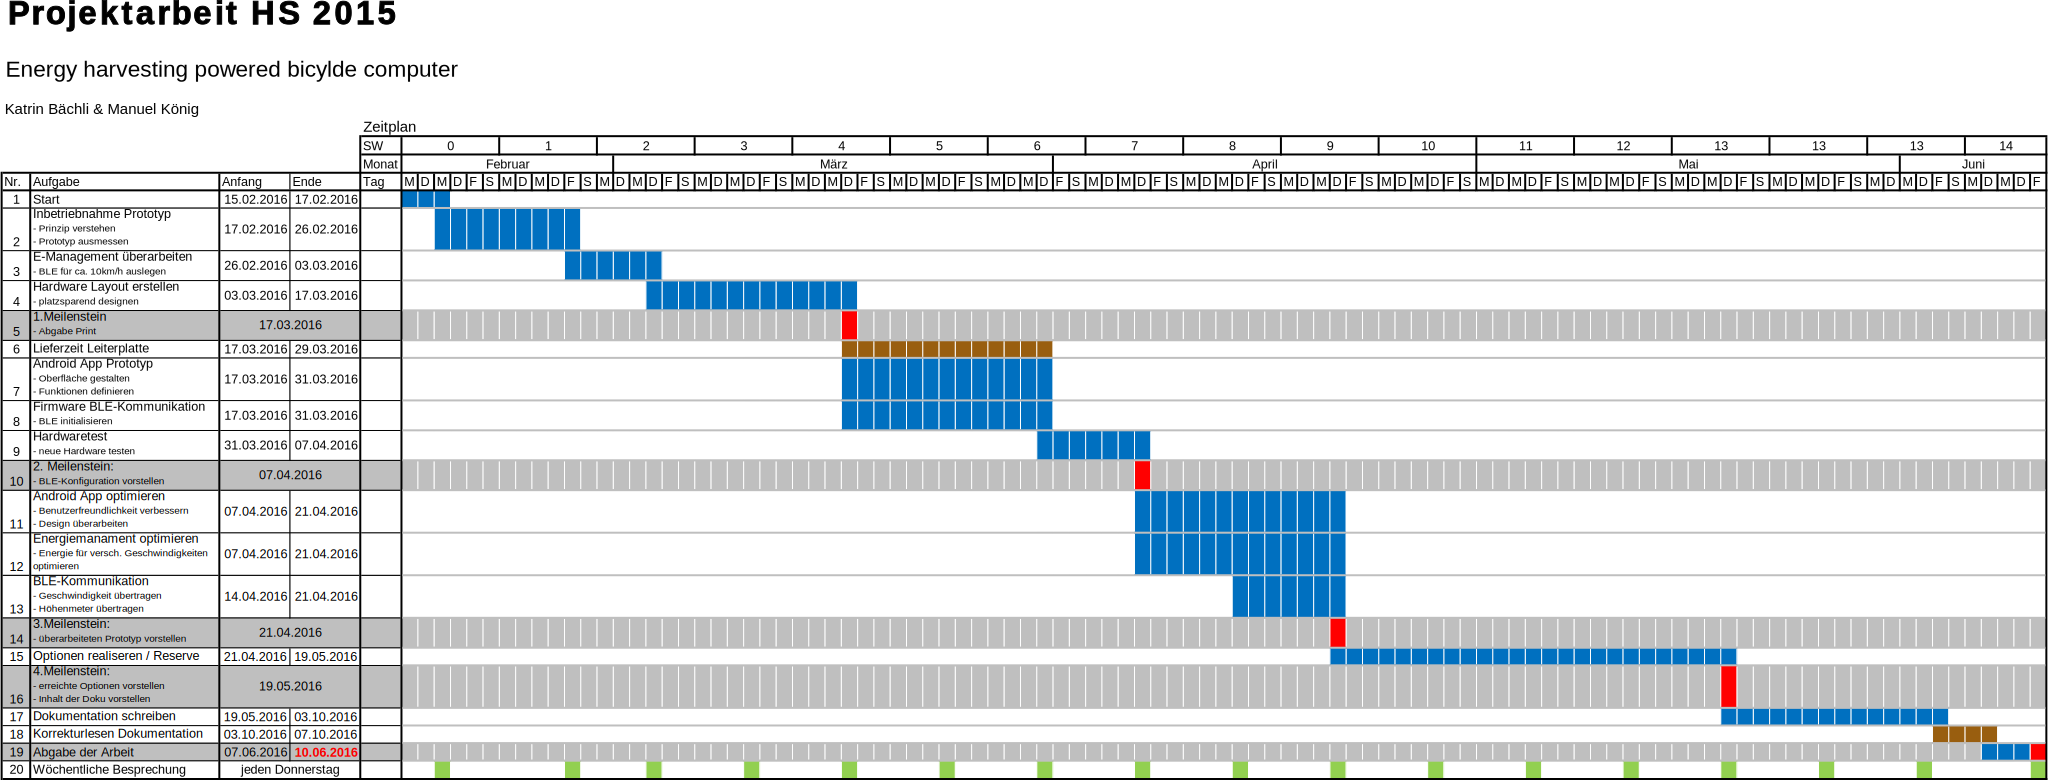
\includegraphics[width=\textheight ,angle=90,origin=c]{../ressources/Projektorganisation/PlannungV0-cropped.pdf}

\chapter{Ausschreibung Bachelorarbeit}

\begin{figure}[h]
    \includegraphics {7Anhang/docs/Ausschreibung.pdf} 
     \caption{Offizielle Ausschreibung der Arbeit}\label{Ausschreibung} 
\end{figure}



\chapter{Blockdiagramm EM8500}\label{anhang_em8500} 
\begin{figure}[h]
    \includegraphics {7Anhang/imag/blockdiagrammEm8500.png} 
     \caption{Blockschema Sensortag}
\end{figure}



\chapter{Funktionsblöcke Sensortag von Texas Instrument}\label{anhang_sensortag} 



\begin{figure}[h]
    \includegraphics {7Anhang/imag/CC26xx_Block_Diagram.png} 
     \caption{Blockschema Sensortag aus \cite{Sensortag_Datasheet}, S.3}
\end{figure}



\chapter{Messaufbau}
\label{messaufbau}
Problematisch war, dass die Messresultate mit dem Fahrrad nicht reproduzierbar waren, daher wurde eine Radimitation erarbeitet. Herr Erich Ruff hat einen Aubau entwickelt, welcher über einen Elektromotor angetrieben wurde, damit konnte die Geschwindigkeit relativ konstant gehalten werden. Die Toleranz der Geschwindigkeit lag bei +/- 1 km/h, was eine grosse Verbesserung gegenüber der bisherigen Vorgehensweise war.
Die Radimitation bestand aus nur einer Speiche, welche nur eine einfache Alustange war. An dieser Alustange waren mehrere Löcher zur Befestigung des Topfmagneten vorhanden.


\begin{figure}[ht]
    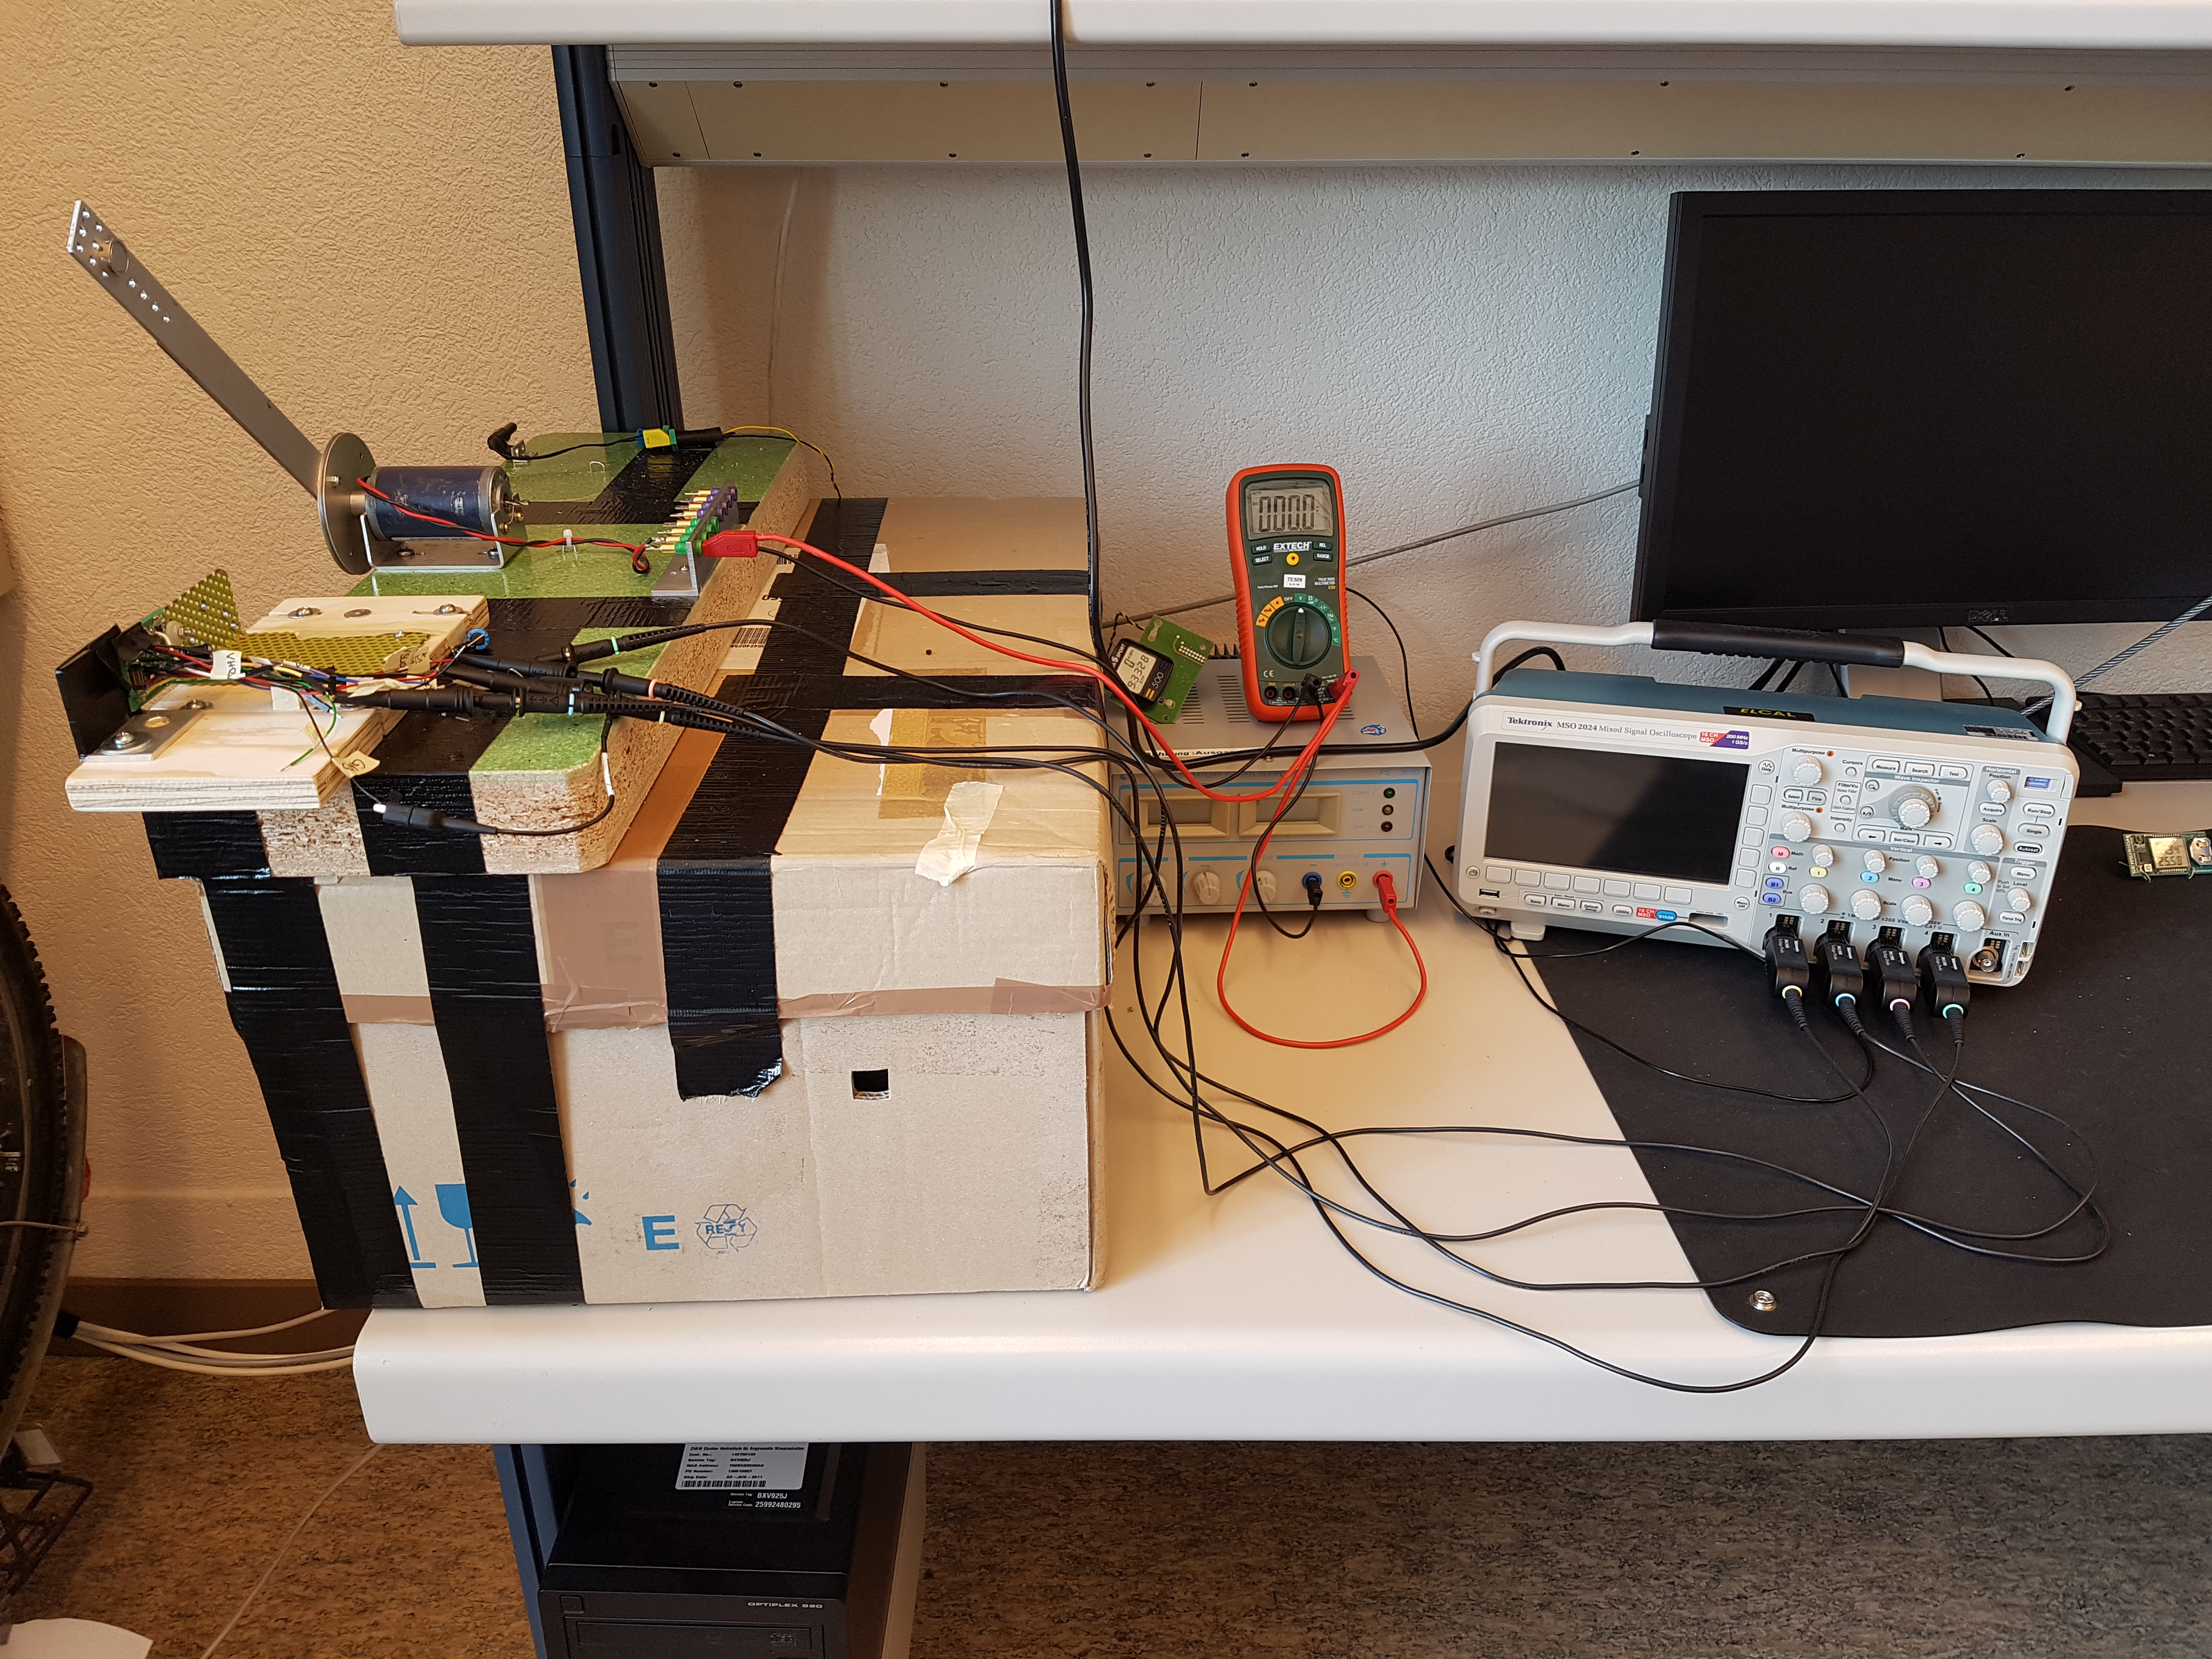
\includegraphics {7Anhang/imag/Messaufbau}
	\caption{Messaufbau während der Inbetriebnahme des Prototypen}
	\label{messaufbau_anhang}
\end{figure}

Der Radimitation ist ein Tachometer angehängt, der die aktuelle Geschwindigkeit anzeigt. Der Tachometer ist vom Hersteller SIGMA Sport, die genaue Bezeichnung Lautet SIGMA SPORT BASELINE 500. Dieser Tachometer wurde im Jahr 1999 hergestellt, funtioniert jedoch nach wie vor einwandfrei.

Im Verlauf der Entwicklung wurde entschieden, dass zwei Magnete im Abstand von 180 Grad angebracht werden. Diese Entscheidung wurde getroffen, um die Energiegewinnung zu maximieren, es wurde jedoch ebenfalls entschieden, dass nicht mehr als zwei Magnete montiert werden sollen. Das Erscheinungbild des Fahrrads würde damit sehr beeinträchtigt und die Bremswirkung würde mit vielen Magneten sicherlich zum Tragen kommen.

\todo{Grad Zeichen einbauen}
\todo{Abstand und Radumfang kontrollieren}
Der Grundabstand ist 25 cm, was einen Radumfang von 2.04 m ergibt. Die ersten Messungen, siehe Anhang \ref{uebersicht_messprotokolle} beziehen sich auf diesen Radumfang. Die Messungen xxx beziehen sich auf einen Radumfang von yyyy.

\chapter{Übersicht Messprotokolle}
\label{uebersicht_messprotokolle}

Aufstellung von Manu
\todo{Messprotokoll Liste}

\subsubsection*{Legende Abbildung  }
\label{bla}
\begin{tabbing}
       Messdatum	   \quad\= Messobjekt    \quad\= Name des PDF     \\[0.8ex]
       xx \> yyy \> name pdf\\
   
\end{tabbing}  




%\chapter{Messprotokoll Energiemessung EM-Chip Ausgang}\label{anhang_messprotokoll_energie_em_chip}\includepdf[pages=-][7Anhang/docs/Messprotokoll_Energiemessung_EM-Ausgang_Dokumentation]

%\chapter{Messprotokoll Energiegewinnung Harvester}\label{anhang_messprotokoll_energie_harvester} 
%\includepdf[pages=-]{../ressources/Energiemessungen/MessungHarvesterschaltungV0.pdf}
%
%
%\chapter{Messprotokoll Energieverbrauch Sensortag}\label{anhang_messprotokoll_energie_sensortag} 
%%\includepdf{../ressources/Projektorganisation/Ausschreibung.pdf}
%
%\chapter{Messprotokoll Rippelspannung Ausgangskondensator Harvesterschaltung}\label{anhang_messprotokoll_kondensator_harvester} 
%\includepdf[pages=-]{../ressources/Energiemessungen/MessungKondensatorAusgang.pdf}